%RSA (Rivest–Shamir–Adleman) is a public-key cryptosystem that is widely used for secure data transmission.
%It is also one of the oldest.
%The acronym RSA comes from the surnames of Ron Rivest, Adi Shamir and Leonard Adleman, who publicly described the
%algorithm in 1977.
%An equivalent system was developed secretly, in 1973 at GCHQ (the British signals intelligence agency), by the
%English mathematician Clifford Cocks.
%That system was declassified in 1997.[1]
%In a public-key cryptosystem, the encryption key is public and distinct from the decryption key, which is kept secret.
%An RSA user creates and publishes a public key based on two large prime numbers, along with an auxiliary value.
%The prime numbers are kept secret.
%Messages can be encrypted by anyone, via the public key, but can only be decoded by someone who knows the prime numbers.
%The security of RSA relies on the practical difficulty of factoring the product of two large prime numbers,
%the "factoring problem".
%Breaking RSA encryption is known as the RSA problem.
%Whether it is as difficult as the factoring problem is an open question.
%There are no published methods to defeat the system if a large enough key is used.
%RSA is a relatively slow algorithm.
%Because of this, it is not commonly used to directly encrypt user data.
%More often, RSA is used to transmit shared keys for symmetric key cryptography, which are then used for bulk
%encryption-decryption.
The RSA algorithm is named after Ron Rivest, Adi Shamir and Len Adleman, who invented it in 1977 [\cite{rivest1978method}].
The basic technique was first discovered in 1973 by Clifford Cocks [\cite{cocks1973note}] of CESG (part of the British GCHQ)
but this was a secret until 1997.
The patent taken out by RSA Labs has expired.

Historically, the process of encryption is considered to be symmetric one.
That means that prior the communication, the sides conclude on the common key to be used in encryption.
This process is similar to the first sharing keys and only after that the locked chest with the message.
Such approach is highly cost since it requires to share the defined keys between each actor if the number of actors
is greater than 2.
Much more simpler is to think about secured communication channel that in terms of asymmetric encryption.
The real life example would be if Alice shares with all actors an opened lock having key.
So that Bob receives an opened lock, writes letter to Alice, puts letter to the chest, locks this chest with received
from Alice lock.
This way, only Alice will be able to open the chest and to read the letter.
This is an idea of the asymmetric encryption.
However, such a simple from first glance idea requires complex number theory approach.
A concept of opened lock may be interpreted in terms of one-way functions.
One way function -- is a function that is easy to compute on every input, but hard to invert given the image of
a random input.
Thus, it is much simpler to close the lock without key, but very difficult to open lock trying the combinations
of the key.
For instance, the function
\begin{equation*}
    f(m) = m^e \bmod N = C
\end{equation*}
where $e, N$ are public constants is one-awy function,
because it is easy to compute $C$ given $m$, however it is hard to compute $m$ given $C$.
So, assume that Alice defines two positive integer constants $e, N$ and sends it to Bob.
Bob encrypts the secret message $m$ using $f(m)$
\[
    f(m) = m^e \bmod N = C
\]
Then Bob sends encrypted message $C$ to the Alice.
Given $C$ Alice must fetch the Bob's message $m$.
In order to decrypt $C$, Alice has to compute
\[
    C^d \bmod N = m^{ed} \bmod N \equiv m,
\]
where $e$ for encryption and $d$ for decryption.
Now the problem is to define such $d$ that it is hard to the listener to fetch it.
In order to define the secret $d$, Alice chooses two enough big prime numbers: $P, \; Q$, let's say around 150 digits
both.
Then Alice multiplies these two prime numbers in order to get $N$
\[
    N = P \cdot Q
\]
The $N$ is around 300 digits.
Now Alice can share $N$ with anyone, since it takes decades to find its prime factorization by the fundamental problem
of prime factorization.
Next, it is very important to know such a function, which depends on the knowledge of factorization of $N$.
Such function is an Euler's totient function.
Given a number $N$ and its prime factorization $p_1^{e_1}\cdot p_2^{e_2} \cdots p_k^{e_k}$, the Euler's totient function
$\phi(N)$ is defined as
\[
    \phi(N) = (p_1^{e_1} - p_1^{e_1 - 1}) \cdot (p_2^{e_2} - p_2^{e_2 - 1}) \cdots (p_k^{e_k} - p_k^{e_k - 1})
\]
In particular, for positive number $M$ such that its factorization is $p1 \cdot p2$, the $\phi(M)$ is
\[
    \phi(M) = (p_1 -1) \cdot (p_2 - 1)
\]
Euler's theorem relates the modular division and exponent as follows, given number $m$, then
\[
    m^{\phi(N)} = 1 \bmod N
\]
It means that reminder of division $m^{\phi(N)}$ by $N$ is always 1.
By the equality $1^K = 1$
\[
    M^{K \cdot \phi(N)} = 1 \bmod N
\]
If we multiply both parts by $M$, we get
\[
    M \cdot M^{K \cdot \phi(N)} = M^{K \cdot \phi(N) + 1} = M \bmod N
\]
It follows that Alice is able to define the secret $d$ as follows
\begin{gather*}
    e \cdot d = K \cdot \phi(N) + 1\\
    d = \frac{K \cdot \phi(N) + 1}{e}\\
\end{gather*}
The following image demonstrates the concept of RSA approach
\begin{figure}[H]
    \centering
    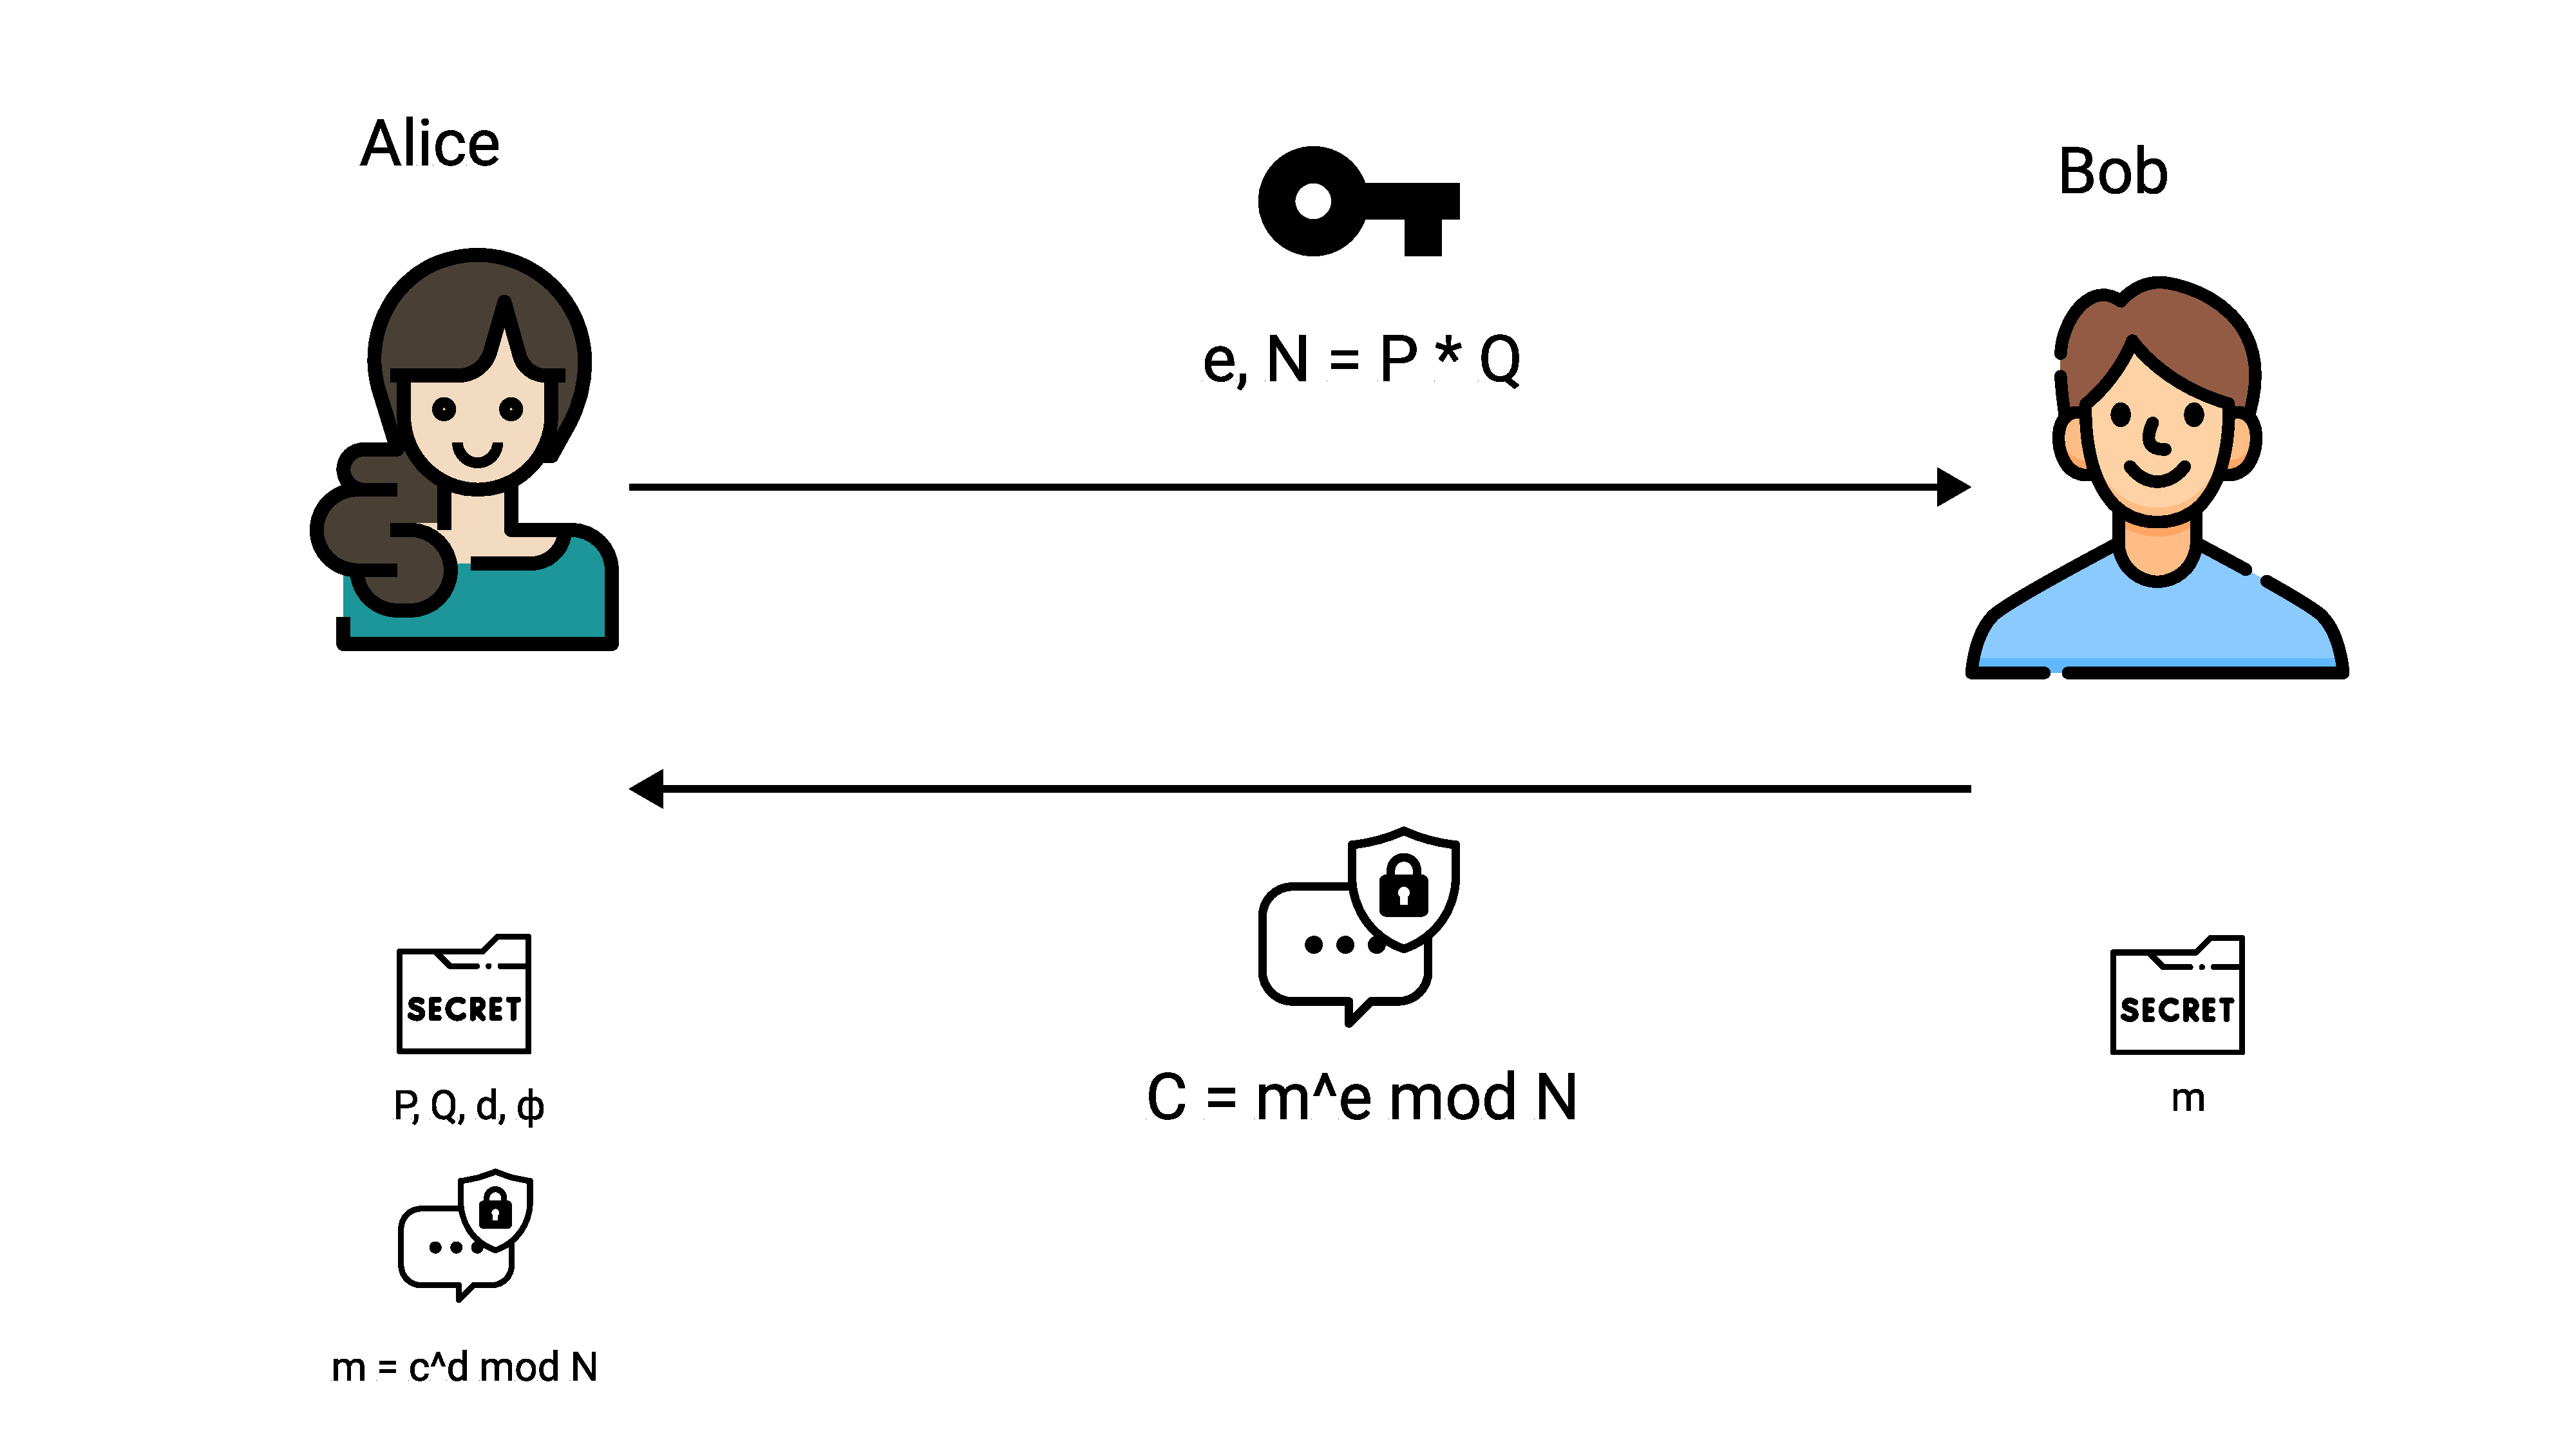
\includegraphics[width=1\textwidth]{Pictures/12_RSA_encryption_concept_diagram}
    \caption{RSA algorithm concept diagram.}\label{fig:figure8}
\end{figure}
To summarize, the process by the steps is as follows
\begin{itemize}
    \item Alice defines the large secret prime numbers $P, \; Q$.
    \item Alice computes $N = P \cdot Q$ and $\phi = (P-1)(Q-1)$
    \item Alice chooses an integer $e$, $1<e< \phi$ such that $\gcd(e, \phi) = 1$.
    \item Alice computes secret exponent $d$, $1<d< \phi$ such that $ed \equiv 1 \bmod \phi$.
    \item Alice shares public key $(N,e)$ with Bob and keeps private key $(d, p, q)$ is secret.
    \item Bob defines the message $m$, encrypts it as $C = m^{e} \bmod N$.
    \item Bob sends $C$ to Alice.
    \item Alice decrypts $C$ using her secret $d$, so she gets $m$
    \[
        m = C^d \bmod N
    \]
\end{itemize}
Security of the RSA approach is based on the complexity of fundamental problem of prime factorization,
which takes decades to solve having enough large number.